\documentclass{beamer}
\usepackage[latin1]{inputenc}

\usetheme{Madrid}
\usecolortheme{default}
\usepackage{amsmath}
\usepackage{amssymb,amsfonts,amsthm}
\usepackage{txfonts}
\usepackage{tkz-euclide}
\usepackage{listings}
\usepackage{adjustbox}
\usepackage{array}
\usepackage{tabularx}
\usepackage{gvv}
\usepackage{lmodern}
\usepackage{circuitikz}
\usepackage{tikz}
\usepackage{graphicx}
\usepackage{gensymb}
\usepackage{physics}

\setbeamertemplate{page number in head/foot}[totalframenumber]

\usepackage{tcolorbox}
\tcbuselibrary{minted,breakable,xparse,skins}



\definecolor{bg}{gray}{0.95}
\DeclareTCBListing{mintedbox}{O{}m!O{}}{%
  breakable=true,
  listing engine=minted,
  listing only,
  minted language=#2,
  minted style=default,
  minted options={%
    linenos,
    gobble=0,
    breaklines=true,
    breakafter=,,
    fontsize=\small,
    numbersep=8pt,
    #1},
  boxsep=0pt,
  left skip=0pt,
  right skip=0pt,
  left=25pt,
  right=0pt,
  top=3pt,
  bottom=3pt,
  arc=5pt,
  leftrule=0pt,
  rightrule=0pt,
  bottomrule=2pt,
  toprule=2pt,
  colback=bg,
  colframe=orange!70,
  enhanced,
  overlay={%
    \begin{tcbclipinterior}
    \fill[orange!20!white] (frame.south west) rectangle ([xshift=20pt]frame.north west);
    \end{tcbclipinterior}},
  #3,
}
\lstset{
    language=C,
    basicstyle=\ttfamily\small,
    keywordstyle=\color{blue},
    stringstyle=\color{orange},
    commentstyle=\color{green!60!black},
    numbers=left,
    numberstyle=\tiny\color{gray},
    breaklines=true,
    showstringspaces=false,
}
\title{4.3.12}
\date{12th september, 2025}
\author{Vishwambhar - EE25BTECH11025}

\begin{document}

\frame{\titlepage}
\begin{frame}{Question}
Check which of the following are solutions of the equation $x-2y=4$ and which are not\\
\begin{enumerate}
    \item $\brak{0,2}$
    \item $\brak{2,0}$
    \item $\brak{4,0}$
    \item $\brak{\sqrt{2},4\sqrt{2}}$
    \item $\brak{1,1}$
\end{enumerate}
\end{frame}

\begin{frame}{Given}
Given line equation can be written as:
\begin{align}
    \vec{n}^\top\vec{x}=c
\end{align}

where $\vec{n}=\myvec{1\\-2}$, $\vec{x}=\myvec{x\\y}$ and $c=4$.\\
\end{frame}

\begin{frame}{Checking}
Checking whether a point lies on the line or not by substituting given vectors in (1):
\begin{align}
    \vec{x}_1=\myvec{0\\2}, \vec{x}_2=\myvec{2\\0}, \vec{x}_3=\myvec{4\\0}, \vec{x}_4=\myvec{\sqrt{2}\\4\sqrt{2}}, \vec{x}_5=\myvec{1\\1}\\
    \vec{n}^\top\myvec{\vec{x}_1&\vec{x}_2&\vec{x}_3&\vec{x}_4&\vec{x}_5}=\myvec{c_1&c_2&c_3&c_4&c_5}\\
    \myvec{1&-2}\myvec{0&2&4&\sqrt{2}&1\\2&0&0&4\sqrt{2}&1}=\myvec{-4&2&4&-7\sqrt{2}&-1}\\
\end{align}

\end{frame}

\begin{frame}{Conclusion}
Conclusion:\\

The point which lies on the line is only option (3).
\end{frame}

\begin{frame}[fragile]
    \frametitle{C Code}
    \begin{lstlisting}
#include<stdio.h>
#include<math.h>
void give_data(double *points){
    points[0] = 1; //Ax
    points[1] = -2; //Ay
    points[2] = 0; //Bx
    points[3] = 2; //By
    points[4] = 2; //Cx
    points[5] = 0; //Cy
    points[6] = 4; //Dx
    points[7] = 0; //Dy
    points[8] = sqrt(2); //EX
    points[9] = 4*sqrt(2); //Ey
    points[10] = 1; //Fx
    points[11] = 1; //Fy
}
    \end{lstlisting}
\end{frame}

\begin{frame}[fragile]
    \frametitle{C Code}
    \begin{lstlisting}
double dotpro(double A[], double B[]){
    double sum = 0;
    for(int i = 0; i<2; i++){
        sum += (A[i]*B[i]);
    }
    return sum;
}
int main(){
    double n[2] = {1, -2};
    double A[2] = {0, 2};
    double B[2] = {2, 0};
    double C[2] = {4, 0};
    double D[2] = {sqrt(2), 4*sqrt(2)};
    double E[2] = {1, 1};
    int k = 0;
    \end{lstlisting}
\end{frame}

\begin{frame}[fragile]
    \frametitle{C Code}
    \begin{lstlisting}
for(int i = 1; i<=5; i++){
        switch (i){case 1: k = dotpro(n, A); if(k==4){printf("Option (%d) lies on the given line.", i);}
            else{printf("Option (%d) does not lie on the given line", i);}
            break;
            case 2: k = dotpro(n, B); if(k==4){printf("Option (%d) lies on the given line.", i);}
            else{printf("Option (%d) does not lie on the given line", i);}
            break;
    \end{lstlisting}
\end{frame}

\begin{frame}[fragile]
    \frametitle{C Code}
    \begin{lstlisting}
            case 3: k = dotpro(n, C); if(k==4){printf("Option (%d) lies on the given line.", i);}
            else{printf("Option (%d) does not lie on the given line", i);}
            break;
            case 4: k = dotpro(n, D); if(k==4){printf("Option (%d) lies on the given line.", i);}
            else{printf("Option (%d) does not lie on the given line", i);}
            break;
            case 5: k = dotpro(n, E); if(k==4){printf("Option (%d) lies on the given line.", i);}
            else{printf("Option (%d) does not lie on the given line", i);}
            break;}}}
    \end{lstlisting}
\end{frame}

\begin{frame}[fragile]
    \frametitle{Python Code 1}
    \begin{lstlisting}
import ctypes as ct

lib = ct.CDLL("./problem.so")

lib.give_data.argtypes = [ct.POINTER(ct.c_double)]

points = ct.c_double*12

data = points()

lib.give_data(data)

def send_data():
    return data[0], data[1], data[2], data[3], data[4], data[5], data[6], data[7], data[8], data[9]
    \end{lstlisting}
\end{frame}

\begin{frame}[fragile]
    \frametitle{Python Code 2}
    \begin{lstlisting}
import matplotlib.pyplot as plt
import numpy as np
import math
from call import send_data
Ax, Ay, Bx, By, Cx, Cy, Dx, Dy, Ex, Ey = send_data()
x = np.linspace(-6, 10, 100)   
y = x/2 - 2
X = [Ax, Bx, Cx, Ex, Dy]
Y = [Ay, By, Cy, Ey, Dy]
plt.plot(x, y, 'r-', label="x-2y=4")
plt.plot(X, Y, 'ko')  

    \end{lstlisting}
\end{frame}

\begin{frame}[fragile]
    \frametitle{Python Code 2}
    \begin{lstlisting}
plt.text(8.17, 1.76, "x-2y=4", fontsize=12, color='black')

for i in range(len(X)-1):
    plt.text(X[i]+0.1, Y[i]+0.1, f"({X[i]:.1f},{Y[i]:.1f})", fontsize=10, color='black')

plt.text(X[4]+0.1, Y[4]+0.1, f"({X[4]:.1f},{Y[4]:.1f})", fontsize=10, color='black')

plt.axvline(x=0, color='k', linewidth=1.5)
    \end{lstlisting}
\end{frame}

\begin{frame}[fragile]
    \frametitle{Python Code 2}
    \begin{lstlisting}
plt.axhline(y=0, color='k', linewidth=1.5)
plt.title("Plot of the given line and points")
plt.xlabel("X-axis")
plt.ylabel("Y-axis")
plt.axis('equal')
plt.grid(True)
plt.savefig("../figs/plot.png")
plt.show()
    \end{lstlisting}
\end{frame}





\begin{frame}{Plot}
    \begin{figure}
        \centering
        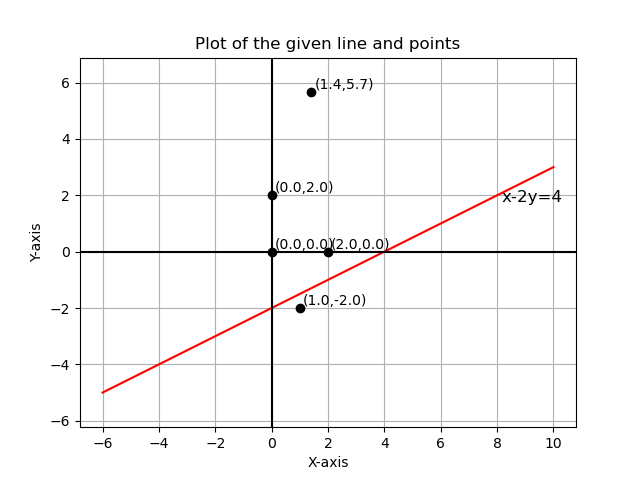
\includegraphics[width=0.5\columnwidth]{../figs/plot.png}
        \caption{Plot of given line and points}
        \label{fig:fig}
    \end{figure}
\end{frame}




\end{document}
